\documentclass{article}\usepackage[]{graphicx}\usepackage[]{color}
% maxwidth is the original width if it is less than linewidth
% otherwise use linewidth (to make sure the graphics do not exceed the margin)
\makeatletter
\def\maxwidth{ %
  \ifdim\Gin@nat@width>\linewidth
    \linewidth
  \else
    \Gin@nat@width
  \fi
}
\makeatother

\definecolor{fgcolor}{rgb}{0.345, 0.345, 0.345}
\newcommand{\hlnum}[1]{\textcolor[rgb]{0.686,0.059,0.569}{#1}}%
\newcommand{\hlstr}[1]{\textcolor[rgb]{0.192,0.494,0.8}{#1}}%
\newcommand{\hlcom}[1]{\textcolor[rgb]{0.678,0.584,0.686}{\textit{#1}}}%
\newcommand{\hlopt}[1]{\textcolor[rgb]{0,0,0}{#1}}%
\newcommand{\hlstd}[1]{\textcolor[rgb]{0.345,0.345,0.345}{#1}}%
\newcommand{\hlkwa}[1]{\textcolor[rgb]{0.161,0.373,0.58}{\textbf{#1}}}%
\newcommand{\hlkwb}[1]{\textcolor[rgb]{0.69,0.353,0.396}{#1}}%
\newcommand{\hlkwc}[1]{\textcolor[rgb]{0.333,0.667,0.333}{#1}}%
\newcommand{\hlkwd}[1]{\textcolor[rgb]{0.737,0.353,0.396}{\textbf{#1}}}%
\let\hlipl\hlkwb

\usepackage{framed}
\makeatletter
\newenvironment{kframe}{%
 \def\at@end@of@kframe{}%
 \ifinner\ifhmode%
  \def\at@end@of@kframe{\end{minipage}}%
  \begin{minipage}{\columnwidth}%
 \fi\fi%
 \def\FrameCommand##1{\hskip\@totalleftmargin \hskip-\fboxsep
 \colorbox{shadecolor}{##1}\hskip-\fboxsep
     % There is no \\@totalrightmargin, so:
     \hskip-\linewidth \hskip-\@totalleftmargin \hskip\columnwidth}%
 \MakeFramed {\advance\hsize-\width
   \@totalleftmargin\z@ \linewidth\hsize
   \@setminipage}}%
 {\par\unskip\endMakeFramed%
 \at@end@of@kframe}
\makeatother

\definecolor{shadecolor}{rgb}{.97, .97, .97}
\definecolor{messagecolor}{rgb}{0, 0, 0}
\definecolor{warningcolor}{rgb}{1, 0, 1}
\definecolor{errorcolor}{rgb}{1, 0, 0}
\newenvironment{knitrout}{}{} % an empty environment to be redefined in TeX

\usepackage{alltt}
\usepackage{Sweave}
\usepackage{float}
\usepackage{graphicx}
\usepackage{tabularx}
\usepackage{siunitx}
\usepackage{amssymb} % for math symbols
\usepackage{amsmath} % for aligning equations
\usepackage{textcomp}
\usepackage{mdframed}
\usepackage{natbib}
\bibliographystyle{/Users/CatherineChamberlain/Documents/git/microclimates/refs/styles/besjournals.bst}
\usepackage[small]{caption}
\setlength{\captionmargin}{30pt}
\setlength{\abovecaptionskip}{0pt}
\setlength{\belowcaptionskip}{10pt}
\topmargin -1.5cm        
\oddsidemargin -0.04cm   
\evensidemargin -0.04cm
\textwidth 16.59cm
\textheight 21.94cm 
%\pagestyle{empty} %comment if want page numbers
\parskip 7.2pt
\renewcommand{\baselinestretch}{1.5}
\parindent 0pt
%\usepackage{lineno}
%\linenumbers

%cross referencing:
\usepackage{xr}
\usepackage{xr-hyper}
\externaldocument{/Users/CatherineChamberlain/Documents/git/microclimates/docs/microclimates_supp}

\newmdenv[
  topline=true,
  bottomline=true,
  skipabove=\topsep,
  skipbelow=\topsep
]{siderules}
\IfFileExists{upquote.sty}{\usepackage{upquote}}{}
\begin{document}

\noindent\textbf{\Large{Understanding growing degree days to predict spring phenology in a warming world}}

\noindent Authors:\\
C. J. Chamberlain $^{1,2}$ \& E. M. Wolkovich $^{1,2,3}$
\vspace{2ex}\\
\emph{Author affiliations:}\\
$^{1}$Arnold Arboretum of Harvard University, 1300 Centre Street, Boston, Massachusetts, USA; \\
$^{2}$Organismic \& Evolutionary Biology, Harvard University, 26 Oxford Street, Cambridge, Massachusetts, USA; \\
$^{3}$Forest \& Conservation Sciences, Faculty of Forestry, University of British Columbia, 2424 Main Mall, Vancouver, BC V6T 1Z4\\
\vspace{2ex}
$^*$Corresponding author: 248.953.0189; cchamberlain@g.harvard.edu\\

\renewcommand{\thetable}{\arabic{table}}
\renewcommand{\thefigure}{\arabic{figure}}
\renewcommand{\labelitemi}{$-$}
\setkeys{Gin}{width=0.8\textwidth}

%%%%%%%%%%%%%%%%%%%%%%%%%%%%%%%%%%%%%%%%%%%%%%%
%%%%%%%%%%%%%%%%%%%%%%%%%%%%%%%%%%%%%%%%%%%%%%%


\section*{Introduction}
\begin{enumerate}
\item Need to start even bigger here! In ecology, we have the fundamental issue of understanding and applying methods to accurately predict shifts in climate and the broader impacts of these shifts.
  \begin{enumerate}
  \item Often we use mixed models to answer ecological questions, though we do not always understand the intricacies of the model output, nor do we investigate what is missing from the model output.
  \item Here, we work to understand mixed models using simulation data and test myriad hypotheses through these simulations. 
  \item These methods can be applied to many ecological questions investigating climate data across global habitats but here we will investigate the effects of climate measurements and site on spring plant phenology. 
  \end{enumerate}
  
\item Understanding and predicting plant phenology in temperate deciduous forests is critical as it both shapes community structure and also influences major ecosystem services such as resource and forest management. 
  \begin{enumerate} 
  \item Climate change and urbanization are advancing spring timing---such as budburst and leafout, which  are strongly cued by temperature, resulting in longer growing seasons \citep{Chuine2001} which ultimately impacts these services.  
  \item Temperate forests sequester carbon and help mitigate the negative effects of climate change and---with earlier spring phenology and longer growing seasons---there has been an increase in carbon uptake \citep{Keenan2014}.
  \item But our understanding of how climate change is impacting this timing of spring is incomplete, especially in urban versus natural forest habitats. 
  \end{enumerate}
  
\item Urbanization has led to the formation of urban heat islands, which have been shown to affect plant phenology and lead to earlier spring leafout \citep{Meng2020}. 
  \begin{enumerate}
  \item These trends are crucial to understand in order to predict plant development with warming. 
  \item Tracking heat accumulation is one way to measure and forecast spring leafout, which is often predicted through the growing degree day (GDD) model \citep{Cook2012,Crimmins2019,Phillimore2013,Schwartz2006,Vitasse2011}.
  \item The GDD model simply sums temperatures above a certain threshold---ideally around 0$^{\circ$C as estimates are proven to be more accurate \citep{Man2010}---and different species often require a different number of GDDs to leaf out. 
  \item GDDs accumulate at a faster rate when mean temperates are higher, thus different sites or different climate measurement methods may record different GDD thresholds for leafout. 
  \item Spring leafout timing can have cascading effects to pollinators \citep{Boggs2012, Pardee2017}, on carbon dynamics \citep{Richardson2013} and albedo \citep{Williamson2016}, thus integrating the growing degree day model successfully is essential for predicting the effects of climate change on temperate systems. 
  \end{enumerate}

\item Phenology is often measured through satellite, remote sensing or PhenoCam images to detect spring `green-up' \citep{Meng2020, Liu2019, Richardson2015} but these methods fail to detect the species---or even site-level---nuances in leafout timing \citep{Elmendorf2019}.
  \begin{enumerate}
  \item Intensive, on the ground observations of individual budburst and leafout timing is the most effective way to implement new methods in calculating growing degree days and predicting future phenology. 
  \item Urban environments additionally provide a natural laboratory for assessing the effects of warming on temperate tree and shrub species as these sites are warming at a faster rate than more rural habitats \citep{Pickett2011, Grimm2008}.
  \end{enumerate}
  
\item Now I want to talk about how arboreta offer another unique lens by incorporating varying provenances and seed sources. 
  \begin{enumerate}
  \item I want to set up this hypothesis here
  \end{enumerate}
  
\item Here I will talk about the differences between using hobo loggers and weather stations
  \begin{enumerate}
  \item I want to set up the two hypotheses here about temperature accuracy.
  \end{enumerate}
  
\item Here, we use both simulations, models and real data to test our hypotheses on modelling GDD accuracy in a warming world.
  \begin{enumerate}
  \item Urban environments require fewer GDDs to leafout than forest habitats.
  \item Individuals with provenance latitudes from more northern locations require fewer GDDs to leafout. 
  \item Hobo loggers are less accurate measures of the same weather as weather stations.
  \item Hobo loggers better capture urban or provenance effects. 
  \end{enumerate}
\end{enumerate}
  

\section*{Methods}
\subsection*{Sites}
\begin{enumerate}
\item We chose two sites---one urban arboretum and one forest---with similar species and climates to compare the number of growing degree days to leafout across species. 
  \begin{enumerate}
  \item The urban site is in Boston, MA at the Arnold Arboretum of Harvard University (42$^{\circ}$17' N -71$^{\circ}$8' W).
  \item The Arnold Arboretum is 281 acres and has a range of elevation of XX to XX
  \item The forest site is in Petersham, MA at the Harvard Forest (42$^{\circ}$31'53.5' N -72$^{\circ}$11'24.1' W).
  \item The Harvard Forest is XXX acres and has a range of elevation of XX to XX. 
  \end{enumerate}
\end{enumerate}

\subsection*{Simulations}

\subsection*{Shiny App}

\subsection*{Data analysis}
\begin{enumerate}
\item Using Bayesian hierarchical models with the rstan package \citep{rstan2019}, version 2.19.2,  in R \citep{R}, version 3.3.1, we estimated the effects of urban or provenance effect and method effect and all two-way interactions as predictors on GDDs until leafout. 
  \begin{enumerate} 
  \item Species were modeled hierarchically as grouping factors, which generates an estimate and posterior distribution of the overall response across the XX species used in our simulations.
  \item We ran four chains, each with 2 500 warm-up iterations and 4 000 sampling iterations for a total of 6 000 posterior samples for each predictor for each model using weakly informative priors.
  \item Increasing priors three-fold did not impact our results.
  \item We evaluated our model performance based on $\hat{R}$ values that were close to one and did not include models with divergent transitions in our results. 
  \item We also evaluated high $n_{eff}$ (4000 for most parameters, but as low as 1400 for a couple of parameters in the shoot apical meristem model). 
  \item We additionally assessed chain convergence and posterior predictive checks visually \citep{BDA}.
  \end{enumerate}
\end{enumerate}
\subsection*{Real Data}
\begin{enumerate}
\item Phenology observations across the Arnold Arboretum were collected by trained citizen scientists from the Tree Spotters National Phenology Network program \citep{NPN}. 
  \begin{enumerate}
  \item The Tree Spotter volunteers observed 15 species with varying phenologies and each species had 5 individuals for a total of 75 trees.


\section*{Results}
\begin{enumerate}
\item Urban environments require fewer GDDs to leafout than forest habitats.
 
\item Individuals with provenance latitudes from more northern locations require fewer GDDs to leafout. 
  
\item Hobo loggers are less accurate measures of the same weather as weather stations.

\item Hobo loggers better capture urban or provenance effects.
  
\item Shiny App 
  
\item Real data 
\end{enumerate}

\section*{Discussion} 
\begin{enumerate}
\item Add section here that discusses why maybe using GDD models may not be appropriate for the future with warming \citep{Man2010}. 
  \begin{enumerate}
  \item This is because with warming, GDDs will accumulate at a faster rate, which will reduce accuracy of determining that actual threshold for leafout phenology. 
  \item In the future, we need to either use a method that is less reliant on accumulated sums---especially if it is a climatilogical sum---or we must scrutinize results through the use of mixed models and simulated data as we demonstrate here. 
  \end{enumerate}
\end{enumerate}




\bibliography{..//refs/micro}

\section*{Tables and Figures}

\iffalse
{\begin{figure} [H]
  -\begin{center}
  -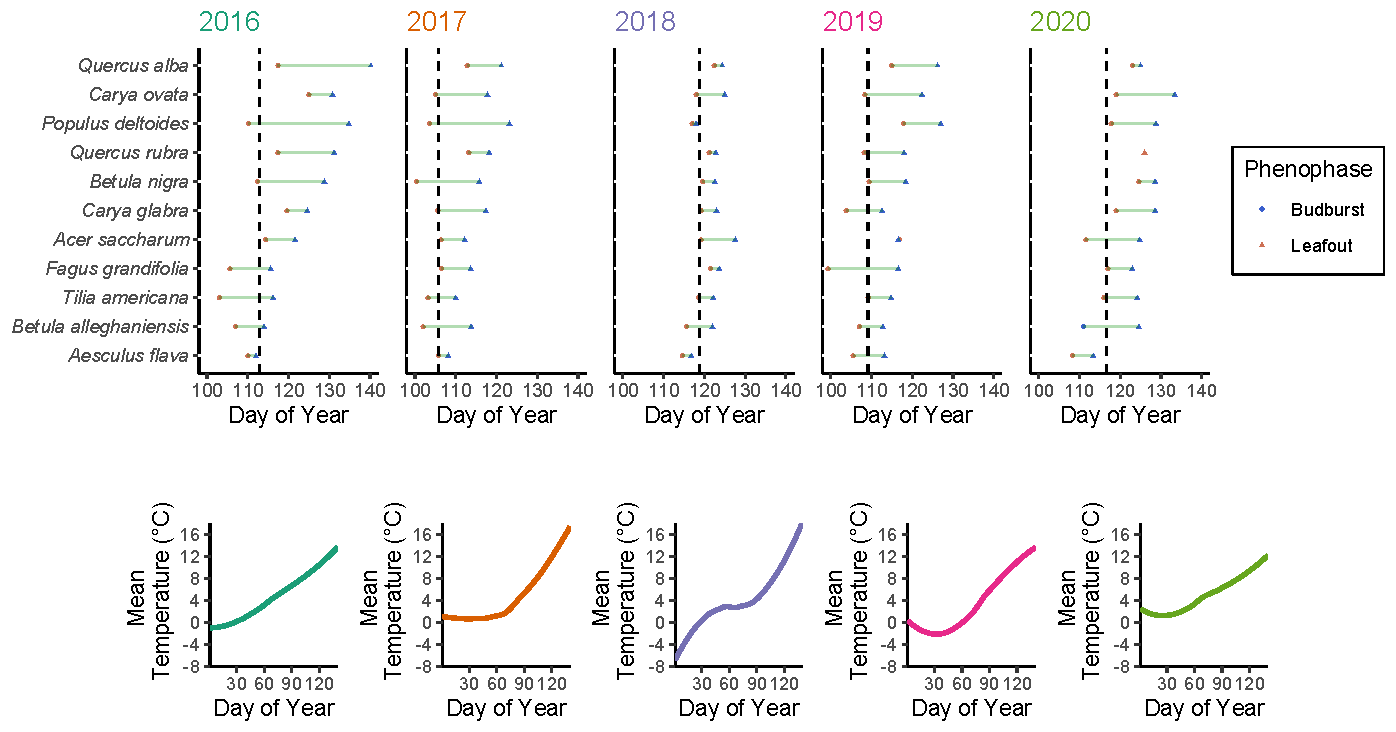
\includegraphics[width=12cm]{..//analyses/figures/dvr_climate_ts.pdf}
  -\caption{}\label{fig:arbclim}
  -\end{center}
  -\end{figure}}

  {\begin{figure} [H]
  -\begin{center}
  -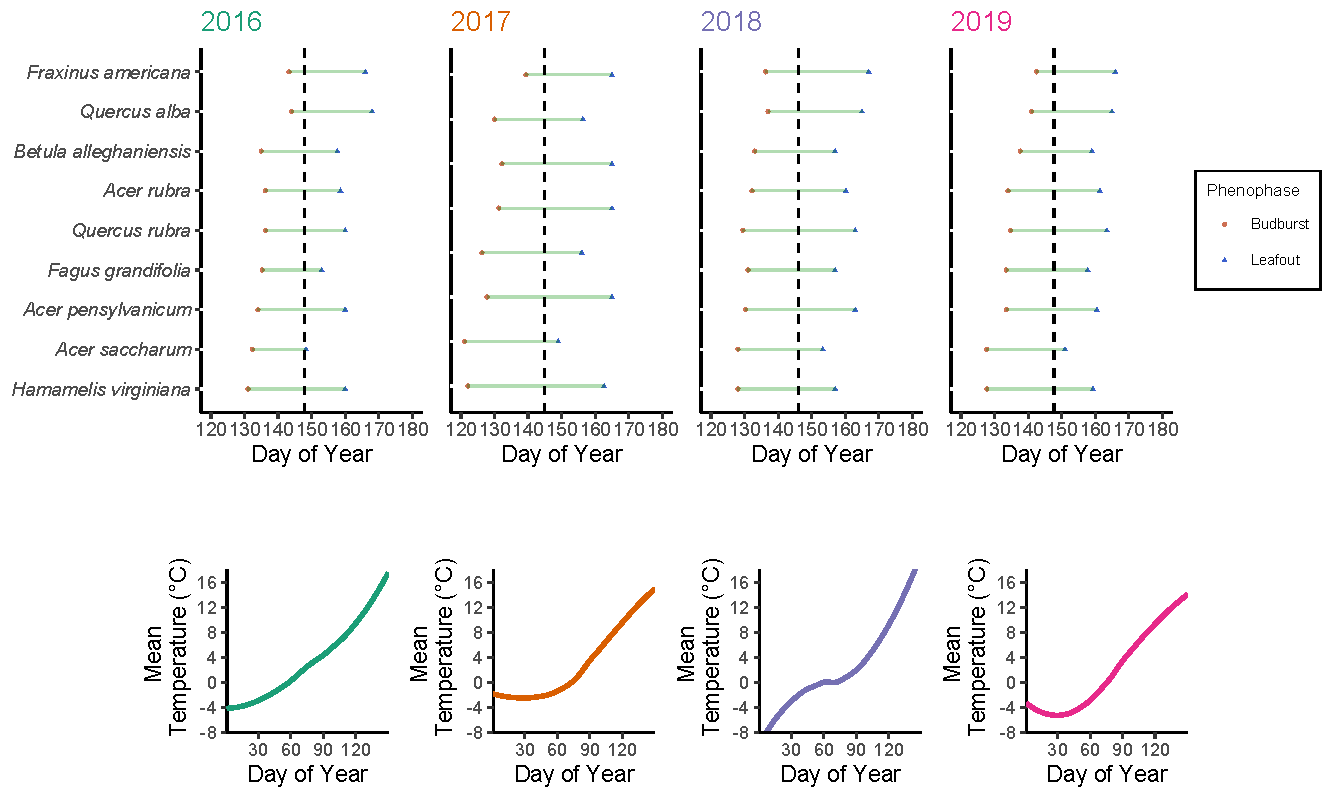
\includegraphics[width=12cm]{..//analyses/figures/dvr_climate_hf.pdf}
  -\caption{}\label{fig:hfclim}
  -\end{center}
  -\end{figure}}
\fi
  
  

\end{document}
